%%
%% This is file `main.tex', based on the generated `sigconf.tex' sample.
%% It was renamed for this project and its bibliography was renamed to
%% `main.bib'.
%%
%% The original source files were:
%%
%% samples.dtx  (with options: `all,proceedings,sigconf')
%% 
%% IMPORTANT NOTICE:
%% 
%% For the copyright see the source file.
%% 
%% Any modified versions of this file must be renamed
%% with new filenames distinct from sigconf.tex.
%% 
%% For distribution of the original source see the terms
%% for copying and modification in the file samples.dtx.
%% 
%% This generated file may be distributed as long as the
%% original source files, as listed above, are part of the
%% same distribution. (The sources need not necessarily be
%% in the same archive or directory.)
%%
%%
%% Commands for TeXCount
%TC:macro \cite [option:text,text]
%TC:macro \citep [option:text,text]
%TC:macro \citet [option:text,text]
%TC:envir table 0 1
%TC:envir table* 0 1
%TC:envir tabular [ignore] word
%TC:envir displaymath 0 word
%TC:envir math 0 word
%TC:envir comment 0 0
%%
%% The first command in your LaTeX source must be the \documentclass
%% command.
%%
%% For submission and review of your manuscript please change the
%% command to \documentclass[manuscript, screen, review]{acmart}.
%%
%% When submitting camera ready or to TAPS, please change the command
%% to \documentclass[sigconf]{acmart} or whichever template is required
%% for your publication.
%%
%%
\documentclass[sigconf]{acmart}
\usepackage{xcolor}
\usepackage{cleveref}
\usepackage{listings}
\lstdefinestyle{c}{
  frame=none,
  xleftmargin=2pt,
  stepnumber=1,
  numbers=left,
  numbersep=5pt,
  numberstyle=\ttfamily\tiny\color[gray]{0.3},
  belowcaptionskip=\bigskipamount,
  captionpos=b,
  escapeinside={*'}{'*},
  language=C,
  keepspaces=true,
  tabsize=2,
  keywordstyle=[1]{\color{purple}},
  keywordstyle=[4]{\color{blue}},
  keywordstyle=[5]{\color{purple!70!black}},
  morekeywords=[1]{
    auto, break, case, const, continue, default, do, else, enum,
    extern, for, goto, if, inline, register, restrict, return,
    signed, sizeof, static, struct, switch, typedef, union, unsigned,
    volatile, while, include, define, ifndef, endif
  },
  morekeywords=[4]{
    int, long, short, void, char, double, float, bool, size_t,
    uint8_t, uint16_t, uint32_t, uint64_t, int8_t, int16_t,
    int32_t, int64_t
  },
  commentstyle=\color{teal},
  stringstyle=\ttfamily,
  delim=[s][\ttfamily\color{orange}]{"}{"},
  columns=flexible,
  basicstyle=\small\ttfamily,
  showspaces=false,
  showstringspaces=false,
}
\lstdefinestyle{make}{
  frame=none,
  xleftmargin=2pt,
  stepnumber=1,
  numbers=left,
  numbersep=5pt,
  numberstyle=\ttfamily\tiny\color[gray]{0.3},
  belowcaptionskip=\bigskipamount,
  captionpos=b,
  language={[gnu]make},
  keepspaces=true,
  tabsize=2,
  keywordstyle=\color{purple},
  identifierstyle=\color{blue!70!black},
  commentstyle=\color{teal},
  stringstyle=\color{orange},
  columns=flexible,
  basicstyle=\small\ttfamily,
  showspaces=false,
  showstringspaces=false,
}
\lstdefinestyle{haskell}{
  frame=none,
  xleftmargin=2pt,
  stepnumber=1,
  numbers=left,
  numbersep=5pt,
  numberstyle=\ttfamily\tiny\color[gray]{0.3},
  belowcaptionskip=\bigskipamount,
  alsoletter={=<>-|{}},
  captionpos=b,
  escapeinside={*'}{'*},
  keywordstyle=[2]{\color{teal}},
  keywordstyle=[3]{\color{violet}},
  keywordstyle=[1]{\bfseries\color{purple}},
  keywordstyle=[4]{\color{blue}},
  keywordstyle=[5]{\color{cyan!50!black}},
  keywordstyle=[6]{\bfseries\color{purple}},
  keywords=[3]{
    INLINE, PRAGMA, NOINLINE, RULES, SPECIALISE, LANGUAGE, forall,
    DataKinds, TypeApplications
  },
  keywords=[4]{
    Int, Bool, Double, Maybe, Either, Monad, Map, String, ByteString,
    IO, Proxy, KnownSymbol, Show, Read, IORef, Num, MVar,
    Word32, Word64, Property, MonadIO, Type, FilePath, Vector,
    Integer, Setup, Secure, Nonsecure, NSEffects, SEffects, EXTI, GPIO,
    UART, Locked, Unlocked, Nil, Cons, N0, N1, N2, N3, N4, N7, N13,
    A, B, C, D, E, F, G, H, EXTIEdge, Member, Delete, Fresh, Periph,
    TZSC, RCC, GPIOActions, UARTActions, NonSecureCallable, Callable,
    NFData
  },
  keywords=[5]{
    True, False, Nothing, Just, Left, Right,
    UARTConfig, GPIOConfig, EXTIConfig,
    NONE, OUTPUT, INPUT, NOPULL, PULLUP, PULLDOWN, AF0,
    BOTH, FALLING, RISING, RCC_GPIOC, RCC_GPIOG
  },
  morekeywords=[1]{
    do, if, then, else, case, of, class, data, newtype, instance,
    where, deriving, import, let, in, module, qualified, type
  },
  morekeywords=[6]{div},
  otherkeywords={<.>, <-, ->, <>, ::, ':, \$, +, [, ],/,\\, \,, =, =>, ==>, |, \{, \}, (, ), -\#, \#-, @},
  morekeywords=[2]{-\#, \#-, \{, \#, \}},
  tabsize=2,
  keepspaces=true,
  comment=[l]{--},
  commentstyle=\color{teal},
  stringstyle=\ttfamily,
  showspaces=false,
  delim=[s][\ttfamily\color{orange}]{"}{"},
  columns=flexible,
  basicstyle=\small\ttfamily,
  showstringspaces=false,
}
\lstdefinestyle{haskellinline}{
  style=haskell,
  columns=fullflexible,
  basicstyle=\ttfamily,
  keywordstyle=[1]{\color{purple}},
}
\lstdefinestyle{cinline}{
  style=c,
  numbers=none,
  xleftmargin=0pt,
  basicstyle=\ttfamily,
  columns=fullflexible,
}
\NewDocumentCommand{\inlinec}{v}{\lstinline[style=cinline]|#1|}
\NewDocumentCommand{\inlinehaskell}{v}{\lstinline[style=haskellinline]|#1|}
\newcommand{\todo}[1]{\textcolor{red}{#1}}
%%
%% \BibTeX command to typeset BibTeX logo in the docs
\AtBeginDocument{%
  \providecommand\BibTeX{{%
    Bib\TeX}}}

%% Rights management information.  This information is sent to you
%% when you complete the rights form.  These commands have SAMPLE
%% values in them; it is your responsibility as an author to replace
%% the commands and values with those provided to you when you
%% complete the rights form.
\setcopyright{acmlicensed}
\copyrightyear{2018}
\acmYear{2018}
\acmDOI{XXXXXXX.XXXXXXX}
%% These commands are for a PROCEEDINGS abstract or paper.
\acmConference[Conference acronym 'XX]{Make sure to enter the correct
  conference title from your rights confirmation email}{June 03--05,
  2018}{Woodstock, NY}
%%
%%  Uncomment \acmBooktitle if the title of the proceedings is different
%%  from ``Proceedings of ...''!
%%
%%\acmBooktitle{Woodstock '18: ACM Symposium on Neural Gaze Detection,
%%  June 03--05, 2018, Woodstock, NY}
\acmISBN{978-1-4503-XXXX-X/2018/06}


%%
%% Submission ID.
%% Use this when submitting an article to a sponsored event. You'll
%% receive a unique submission ID from the organizers
%% of the event, and this ID should be used as the parameter to this command.
%%\acmSubmissionID{123-A56-BU3}

%%
%% For managing citations, it is recommended to use bibliography
%% files in BibTeX format.
%%
%% You can then either use BibTeX with the ACM-Reference-Format style,
%% or BibLaTeX with the acmnumeric or acmauthoryear sytles, that include
%% support for advanced citation of software artefact from the
%% biblatex-software package, also separately available on CTAN.
%%
%% Look at the sample-*-biblatex.tex files for templates showcasing
%% the biblatex styles.
%%
%%
%% The majority of ACM publications use numbered citations and
%% references.  The command \citestyle{authoryear} switches to the
%% "author year" style.
%%
%% If you are preparing content for an event
%% sponsored by ACM SIGGRAPH, you must use the "author year" style of
%% citations and references.
%% Uncommenting
%% the next command will enable that style.
%%\citestyle{acmauthoryear}


%%
%% end of the preamble, start of the body of the document source.
\begin{document}

%%
%% The "title" command has an optional parameter,
%% allowing the author to define a "short title" to be used in page headers.
\title{MicroHasTEE: Bare-Metal Haskell for Type-Level Peripheral Ownership on TrustZone-M}
\subtitle{A Framework Realized on STM32 Nucleo Boards}

%%
%% The "author" command and its associated commands are used to define
%% the authors and their affiliations.
%% Of note is the shared affiliation of the first two authors, and the
%% "authornote" and "authornotemark" commands
%% used to denote shared contribution to the research.
\author{Robert Krook}
\email{krookr@chalmers.se}
\affiliation{%
  \institution{Chalmers University of Technology and The University of Gothenburg}
  \city{Gothenburg}
  \country{Sweden}
}

%%
%% The abstract is a short summary of the work to be presented in the
%% article.
\begin{abstract}
blabla
\end{abstract}

%%
%% The code below is generated by the tool at http://dl.acm.org/ccs.cfm.
%% Please copy and paste the code instead of the example below.
%%
\begin{CCSXML}
\end{CCSXML}

%%
%% Keywords. The author(s) should pick words that accurately describe
%% the work being presented. Separate the keywords with commas.
\keywords{Do, Not, Use, This, Code, Put, the, Correct, Terms, for,
  Your, Paper}


\received{20 February 2007}
\received[revised]{12 March 2009}
\received[accepted]{5 June 2009}

%%
%% This command processes the author and affiliation and title
%% information and builds the first part of the formatted document.
\maketitle


\section{Introduction}

Arm TrustZone for Armv8-M, or TrustZone-M, partitions a microcontroller into hardware-isolated Secure and Non-secure states.
It also lets Secure firmware expose explicitly declared entry points to Non-secure code.
TrustZone-M does not, however, determine which state owns each peripheral, GPIO pin, or SRAM region.
Vendors implement these assignments through device-specific security hardware.
On the STM32U5 Nucleo board used in this work, memory-mapped security registers, including those of ST's Global TrustZone Controller (GTZC), encode the security attribution of peripherals and SRAM.
Transferring a resource between states therefore requires developers to update this STM32-specific configuration and keep initialization, interrupt routing, and access permissions consistent with it.

Conventional STM32 development turns this configuration into a coordination problem between two separately built firmware images.
Each image can type-check while relying on assumptions about resource ownership that conflict with those of the other image.
Secure code may continue to use a UART after the firmware has assigned it to the Non-secure state, or Non-secure code may assume access to a GPIO pin that the Secure configuration never released.
The hardware enforces the configured boundary at run time, but it cannot determine whether the two applications agree about that boundary.
Developers therefore discover many configuration mismatches only when they execute the firmware on the target device.

MicroHasTEE instead treats TrustZone firmware as a multiparty Haskell program whose participants are the Secure and Non-secure applications.
Although these participants execute as separate firmware images, the programmer implements them simultaneously in one source-level program.
This program describes the computations performed by each participant, the resources available to them, the transfer of resources between them, and their permitted cross-boundary calls.
MicroHs~\cite{augustsson2024microhs} compiles the shared program separately for each TrustZone state.
Each resulting image contains the MicroHs runtime and executes compiled Haskell application code directly on the microcontroller without an operating system or RTOS.
A small C layer provides startup and raw peripheral access, while the application logic, resource partitioning, and cross-state interactions are expressed and executed as Haskell computations.
To the best of our knowledge, MicroHasTEE is the first framework to execute Haskell in both states of a bare-metal TrustZone-M microcontroller and to use a single typed Haskell program to coordinate their resource assignments and cross-state interactions.

This shared description lets MicroHasTEE check assumptions that would remain unrelated in separately written applications.
The type checker verifies that each participant uses only the resources currently available to it and that both participants agree on resource transfers.
It also checks cross-boundary calls against the Secure functions exposed to the Non-secure participant.
Both images are therefore checked against one account of their shared hardware and interface, rather than only being checked in isolation.
A disagreement becomes a compile-time error instead of a fault observed after deployment.

These guarantees apply to operations expressed through MicroHasTEE.
The framework cannot account for arbitrary C or FFI code that accesses a peripheral directly or modifies security registers outside its interface.
The MicroHasTEE programming model is not specific to the STM32U5.
It can target other TrustZone-M microcontrollers with sufficient flash and SRAM, provided that a backend realizes the required memory, peripheral, and interrupt attribution mechanisms.
The implementation evaluated in this work uses the STM32U5-specific security hardware.

This work makes three contributions:

\begin{itemize}
  \item \textbf{A multiparty programming model for TrustZone-M firmware.}
  MicroHasTEE lets developers implement Secure and Non-secure applications together as participants in one source-level program and then compile that program into separate firmware images.

  \item \textbf{Static agreement about resources and cross-boundary interfaces.}
  MicroHasTEE checks each participant's resource use against a shared account of resource authority, transfers, and permitted calls, allowing it to reject inconsistencies before the firmware reaches the target device.

  \item \textbf{Bare-metal Haskell in both TrustZone-M states.}
  The prototype embeds the MicroHs runtime in each firmware image and executes compiled Haskell application code in both states without an operating system or RTOS.
  It connects the high-level shared resource description to the STM32 security configuration and hand-written peripheral drivers.
\end{itemize}

\section{Conventional Bare-Metal TrustZone-M Development}

Constructing a conventional bare-metal TrustZone-M system requires the programmer to express one security partition through several independent hardware and software mechanisms.
THis section first introduces the mechanisms defined by Armv8-M and then explains how STM32 microcontrollers supplement them with device-specific controls for memory, peripherals, and interrupts.
Together, these mechanisms form the low-level programming model that MicroHasTEE seeks to make safer.

\subsection{Memory Partitioning}

A microcontroller contains fixed amounts of flash memory and SRAM, each of which may comprise several physical banks.
A linker script assigns a firmware image to address ranges and places its vector table, code, static data, and stack within them.
\Cref{fig:memory-partition}(a) shows this layout for a conventional bare-metal application.
Because Secure and Non-secure firmware are built as separate images, each image requires its own linker script.
The Secure linker script must also reserve a Non-secure Callable region for the gateway veneers used to enter Secure code.

TrustZone-M allows developers to partition memory into Secure and Non-secure regions.
Our implementation assigns one primary flash range and one primary SRAM range to each security state and reserves a Non-secure Callable subregion within Secure flash.
The MCU's alignment and block-size requirements constrain the boundaries of these regions.
As \cref{fig:memory-partition}(b) shows, the two firmware images occupy disjoint regions of the same physical flash and SRAM.

The linker scripts describe this intended layout, but they do not enforce its security attributes.
Secure startup code must configure the architectural and STM32-specific attribution mechanisms to enforce the same partition.
The two images can therefore link successfully even when the linker and hardware configurations disagree.
Such a mismatch typically triggers a fault only when firmware accesses the affected region.

On the STM32U5, ST's \textit{Implementation Defined Attribution Unit} (IDAU) assigns fixed security attributes to address ranges.
The Cortex-M33 supplements this fixed mapping with a programmable \textit{Security Attribution Unit} (SAU).
For each CPU access, the processor combines the IDAU and SAU results and selects the more restrictive attribute.
The processor orders these attributes as Secure \(>\) Secure, Non-secure Callable \(>\) Non-secure.

The IDAU and SAU classify only transactions issued by the CPU, while other bus masters can access SRAM without passing through them.
ST therefore protects each SRAM bank at its memory interface with a block-based memory protection controller (MPCBB).
Each MPCBB assigns Secure or Non-secure attributes to individual SRAM blocks.
The SAU/IDAU and MPCBB configurations must assign compatible attributes to every SRAM region used by the firmware.

\begin{figure*}[t]
  \centering
  \begin{minipage}[c]{0.43\textwidth}
    \centering
    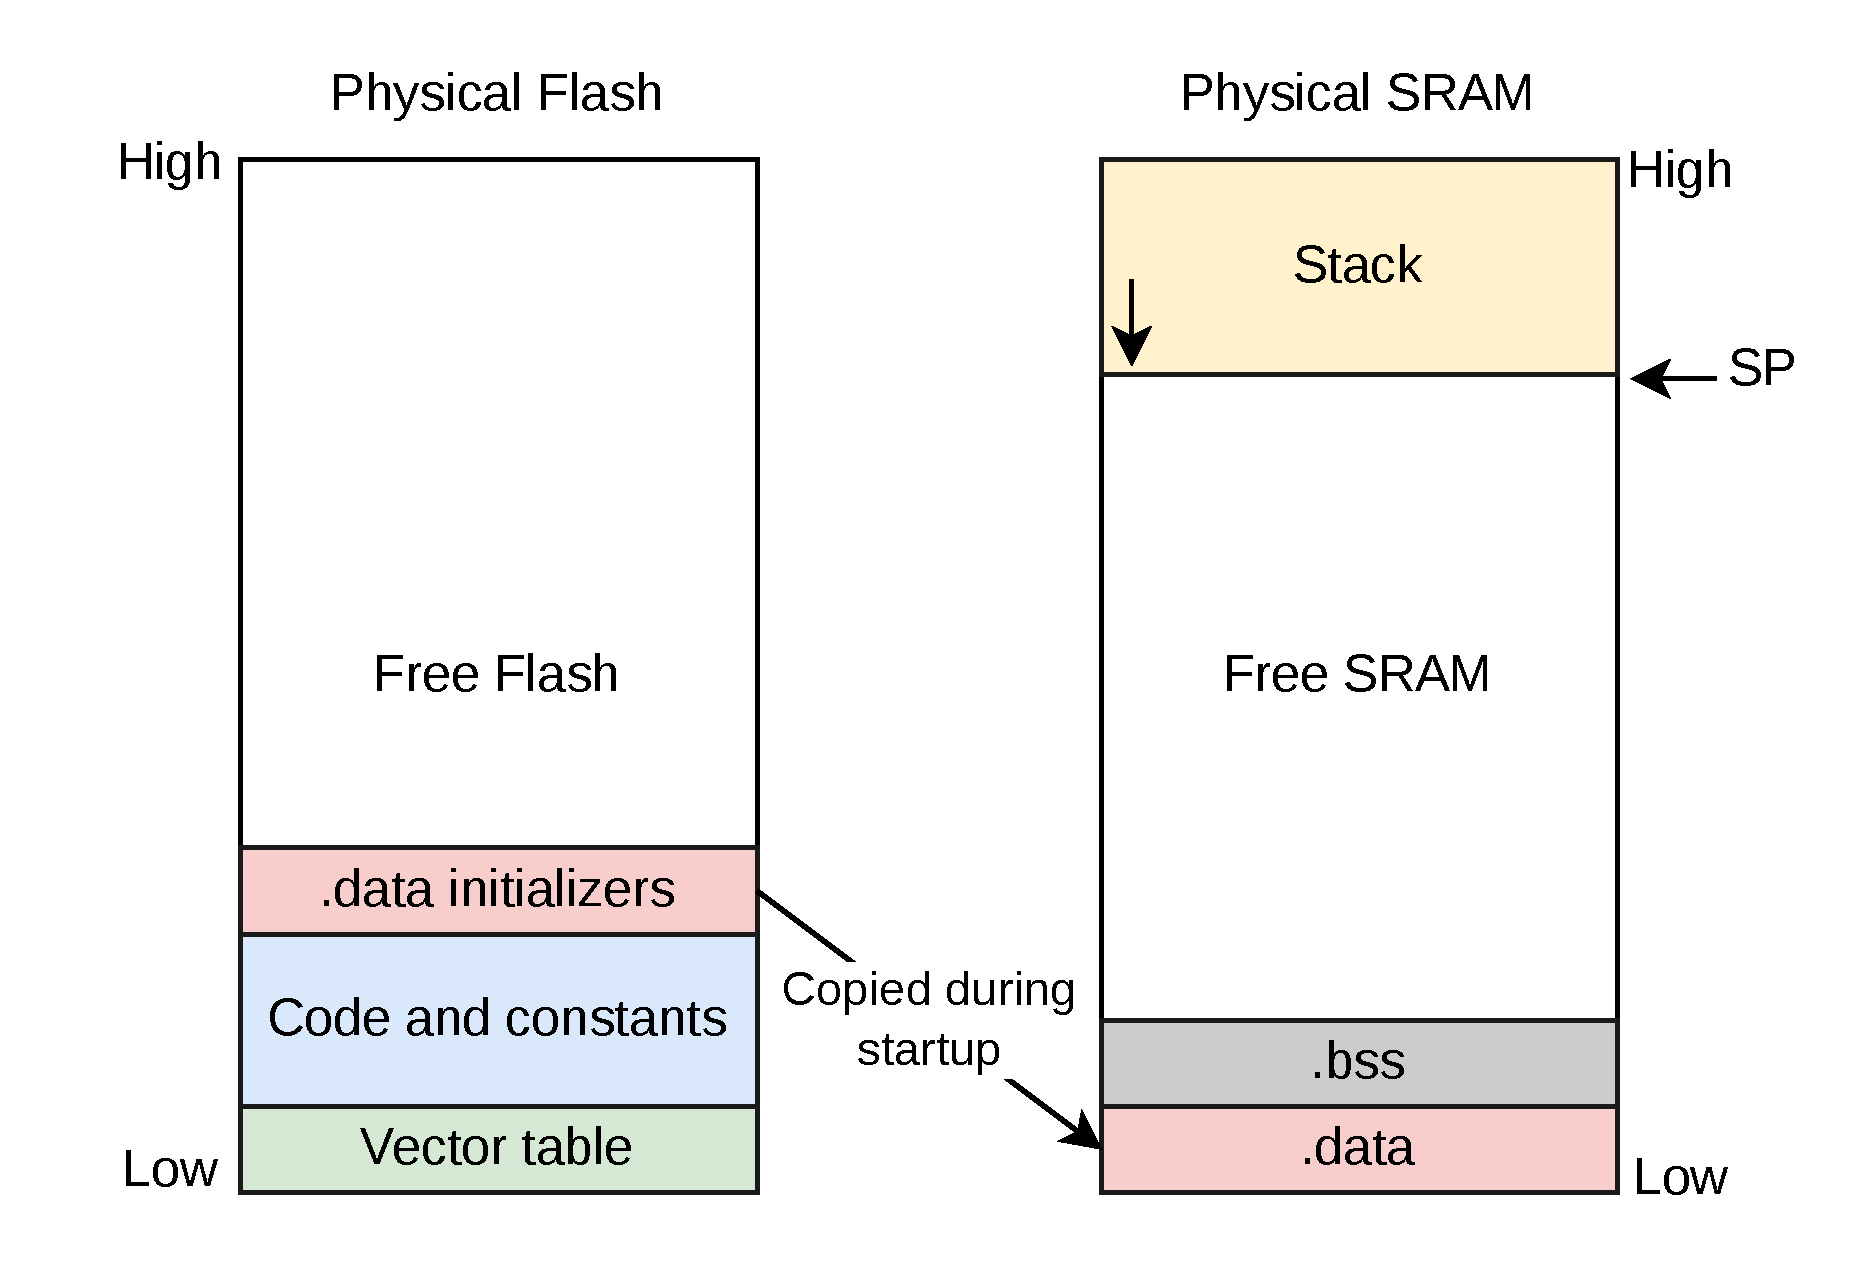
\includegraphics[width=\linewidth]{graphics/microhastee-single-app.drawio.pdf}
    \par\smallskip
    \textbf{(a)} Single application
  \end{minipage}\hfill
  \begin{minipage}[c]{0.54\textwidth}
    \centering
    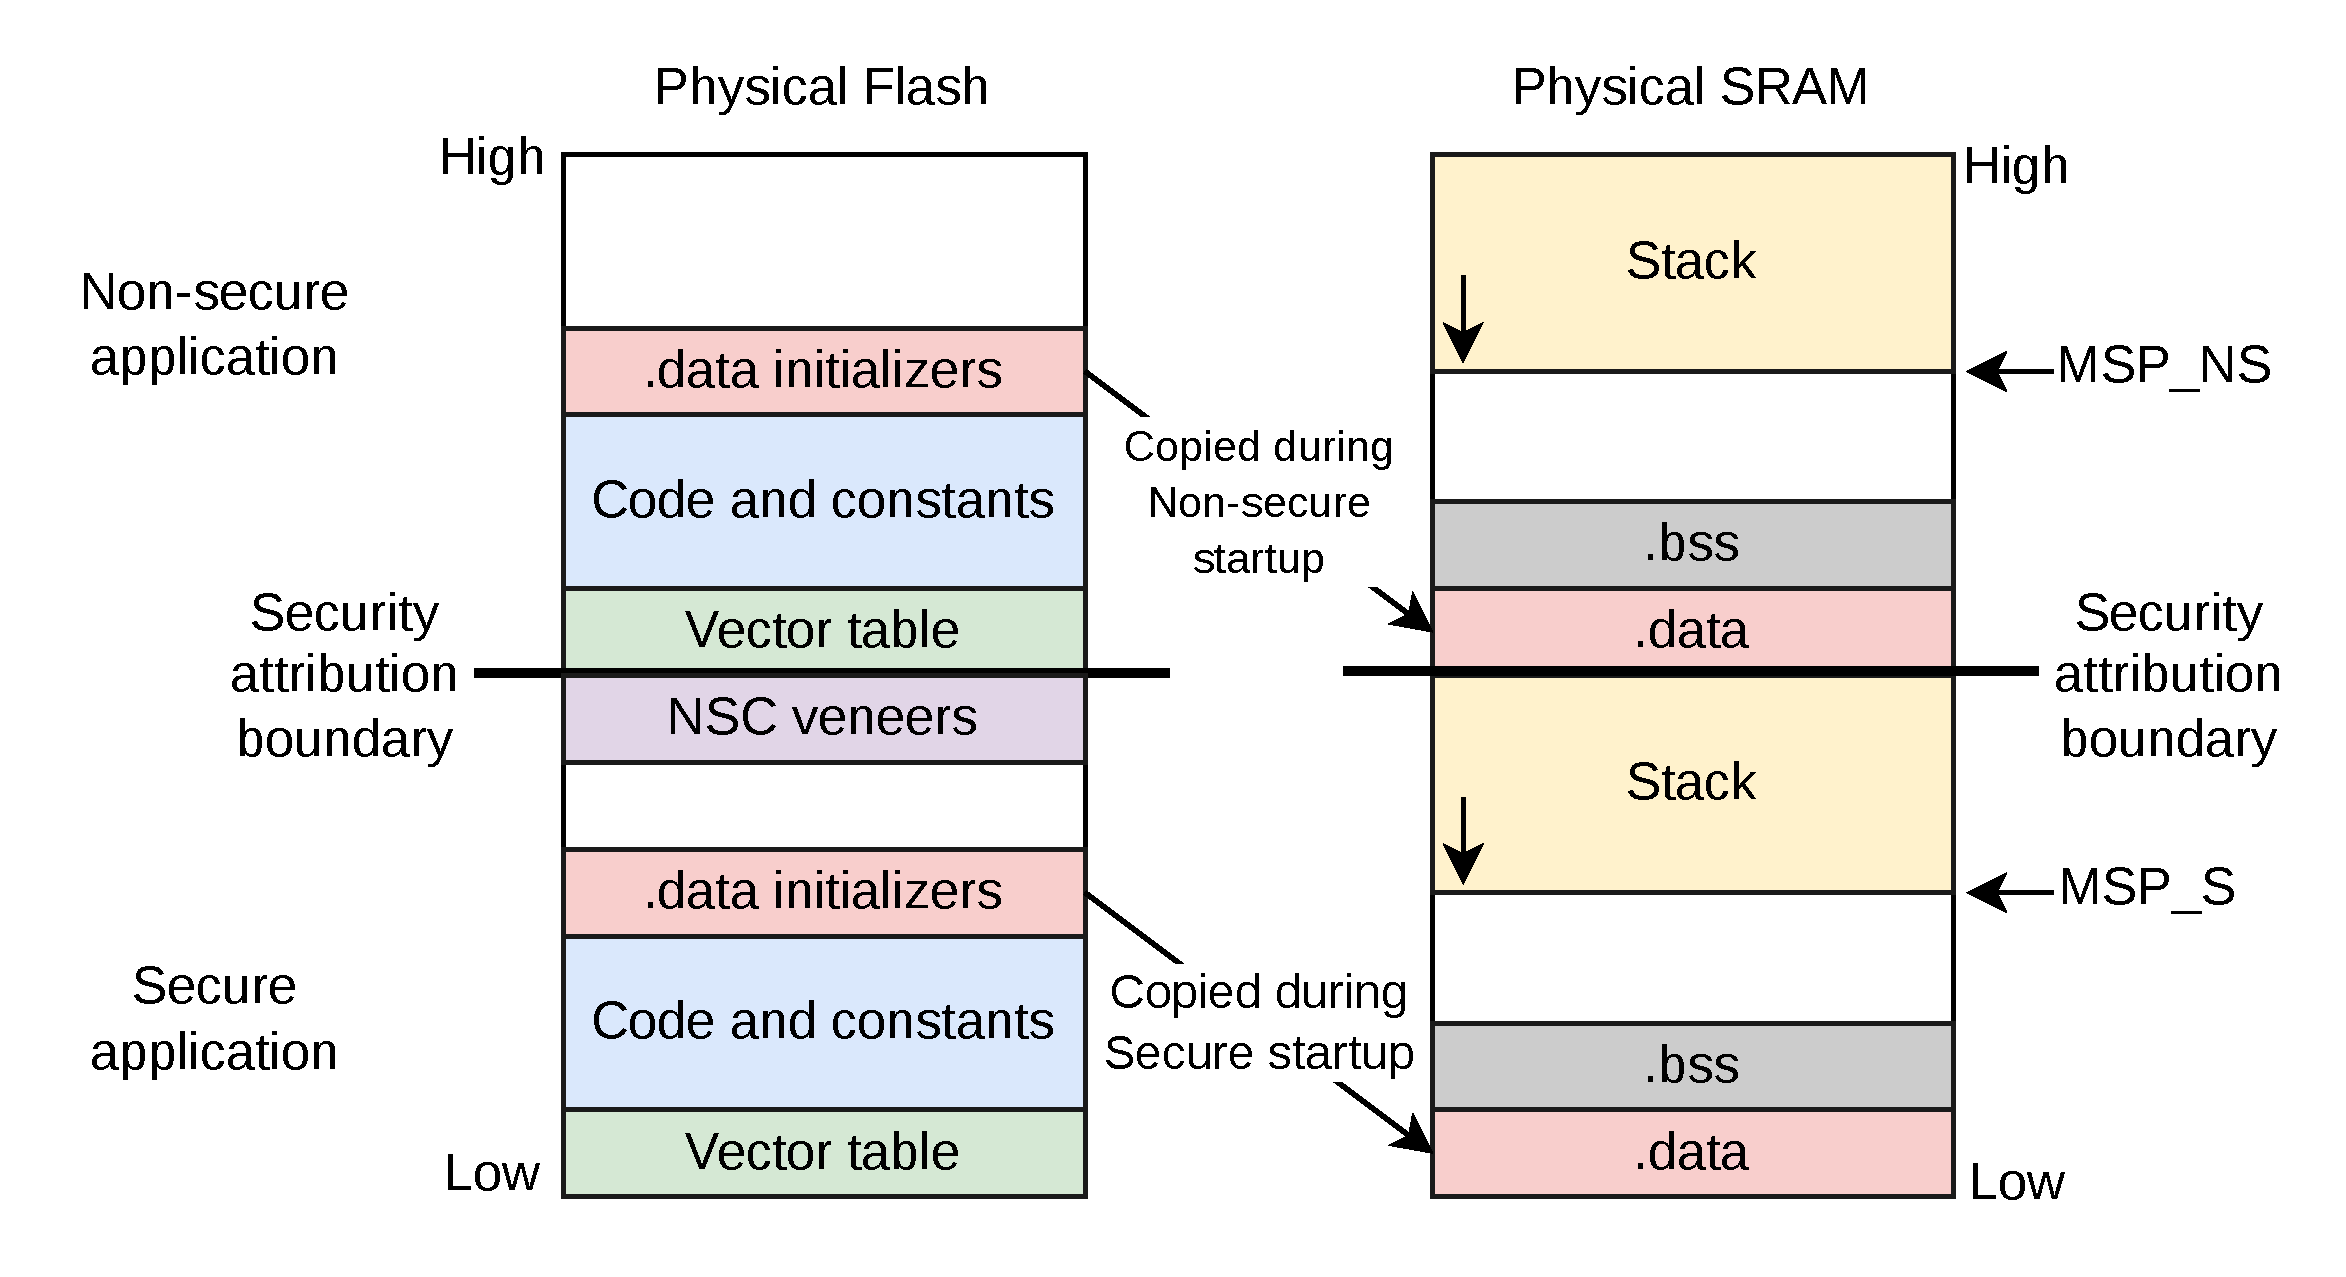
\includegraphics[width=\linewidth]{graphics/microhastee-double-app.drawio.pdf}
    \par\smallskip
    \textbf{(b)} Secure and Non-secure applications
  \end{minipage}
  \caption{Physical flash and SRAM layouts for a single bare-metal application and two TrustZone-M applications.
  The layouts are not drawn to scale.}
  \Description{Side-by-side memory maps compare a single bare-metal application with Secure and Non-secure applications partitioned across the same physical flash and SRAM.}
  \label{fig:memory-partition}
\end{figure*}

\subsection{Peripheral Attribution with the GTZC}

Armv8-M defines the Secure and Non-secure states, memory attribution, and the mechanisms for transferring control between the two states.
STM32 microcontrollers supplement these architectural mechanisms with controls that assign security attributes to memory-mapped peripherals.
The \textit{Global TrustZone Controller} (GTZC) includes a \textit{TrustZone Security Controller} (TZSC), which configures the security attribution of supported peripherals.
Although the GTZC provides additional protection and monitoring mechanisms, we focus here on the TZSC's role in peripheral attribution.

Each peripheral controlled by the TZSC has a corresponding bit in a security configuration register.
A Secure attribution blocks Non-secure transactions, whereas a Non-secure attribution permits them.
A Non-secure attribution therefore does not give the Non-secure state exclusive access to the peripheral.

Some STM32 peripherals provide finer-grained attribution through their own security registers.
For example, each GPIO port controls up to 16 pins and provides a security configuration bit for each implemented pin.
Secure software can therefore retain Secure access to selected pins while permitting Non-secure access to other pins on the same port.
Only Secure software can modify these security attributes.

\subsection{Interrupt Attribution}

Peripheral attribution does not by itself determine where interrupts from that peripheral execute.
Armv8-M assigns each external interrupt a target security state through the Interrupt Target Non-secure State (\texttt{ITNS}) registers in the Nested Vectored Interrupt Controller (NVIC).
Secure software configures this target, and the processor uses either the Secure or the Non-secure vector table when it takes the interrupt.

STM32 devices may also attribute the interrupt source independently of its NVIC target.
For example, moving a button input to the Non-secure application requires Secure firmware to make the GPIO pin Non-secure, configure the corresponding EXTI line and mark it Non-secure, and target its NVIC interrupt to the Non-secure state.
The Non-secure image must also contain a handler in the corresponding slot of its vector table.
These settings must agree before the interrupt is enabled.
Releasing the GPIO pin alone is therefore insufficient: if the EXTI attribution, NVIC target, or vector entry disagrees, the event may be delivered to the wrong state or to a handler that cannot service it.

\subsection{Non-secure Callable Functions and Gateway Veneers}

The Secure and Non-secure firmware images occupy disjoint regions of flash and SRAM.
This isolation is asymmetric: Secure software can access Non-secure resources, whereas Non-secure software cannot directly access Secure memory or peripherals.
Secure firmware can nevertheless expose selected entry functions to Non-secure callers without exposing its remaining code and data.

Secure firmware declares an entry function using the CMSE \inlinec{cmse_nonsecure_entry} attribute.
The compiler marks the function as a Secure entry point, and the Secure linker creates a corresponding secure gateway veneer in a Non-secure Callable region.
The veneer consists of an \texttt{SG} instruction followed by a branch to the entry function in Secure memory.
Non-secure code calls the exported gateway symbol as an ordinary function.
When the processor executes \texttt{SG} at a valid gateway, it changes to the Secure state and continues to the entry function.
The compiler-generated epilogue clears register state as required and executes \texttt{BXNS} to return directly to the Non-secure caller.

Below is a simple function defined by the Secure application, with an attribute that marks it as a NSC function.

\begin{lstlisting}[style=c]
int __attribute__((cmse_nonsecure_entry))
add10(int value) {
  return value + 10;
}
\end{lstlisting}

The Non-secure application declares the function and calls it like an ordinary external function.
THe linker will resolve it when the firmware is built.

\begin{lstlisting}[style=c]
extern int add10(int value);

int myadd(void) {
  return add10(5);
}
\end{lstlisting}

This declaration is sufficient to compile the Non-secure source, but it is not sufficient to link the Non-secure image.
The address associated with \inlinec{add10} is the address of the gateway veneer created when the Secure image is linked.
With the GNU toolchain, the Secure link uses \texttt{--cmse-implib} and \texttt{--out-implib} to emit a CMSE import library containing the exported symbols and their veneer addresses.
The Non-secure linker must then consume this generated library.

The simplified build dependency is therefore:

\begin{lstlisting}[style=make]
secure.elf:
	$(CC) ... -Wl,--cmse-implib,\
	            --out-implib=secure_cmse_import.lib

nonsecure.elf: secure.elf
	$(CC) ... secure_cmse_import.lib
\end{lstlisting}

The two images are linked separately, but they cannot be built independently.
The Secure link must run first, and any change to the exposed interface or veneer placement requires the import library and Non-secure image to be regenerated together.
Moreover, the C linker resolves \inlinec{add10} by symbol name and address; it does not verify that the independently compiled declarations on the two sides have matching types.

The control flow of this call from Non-secure to Secure code is shown in \cref{fig:nsc-call}.

\begin{figure}[ht]
  \centering
  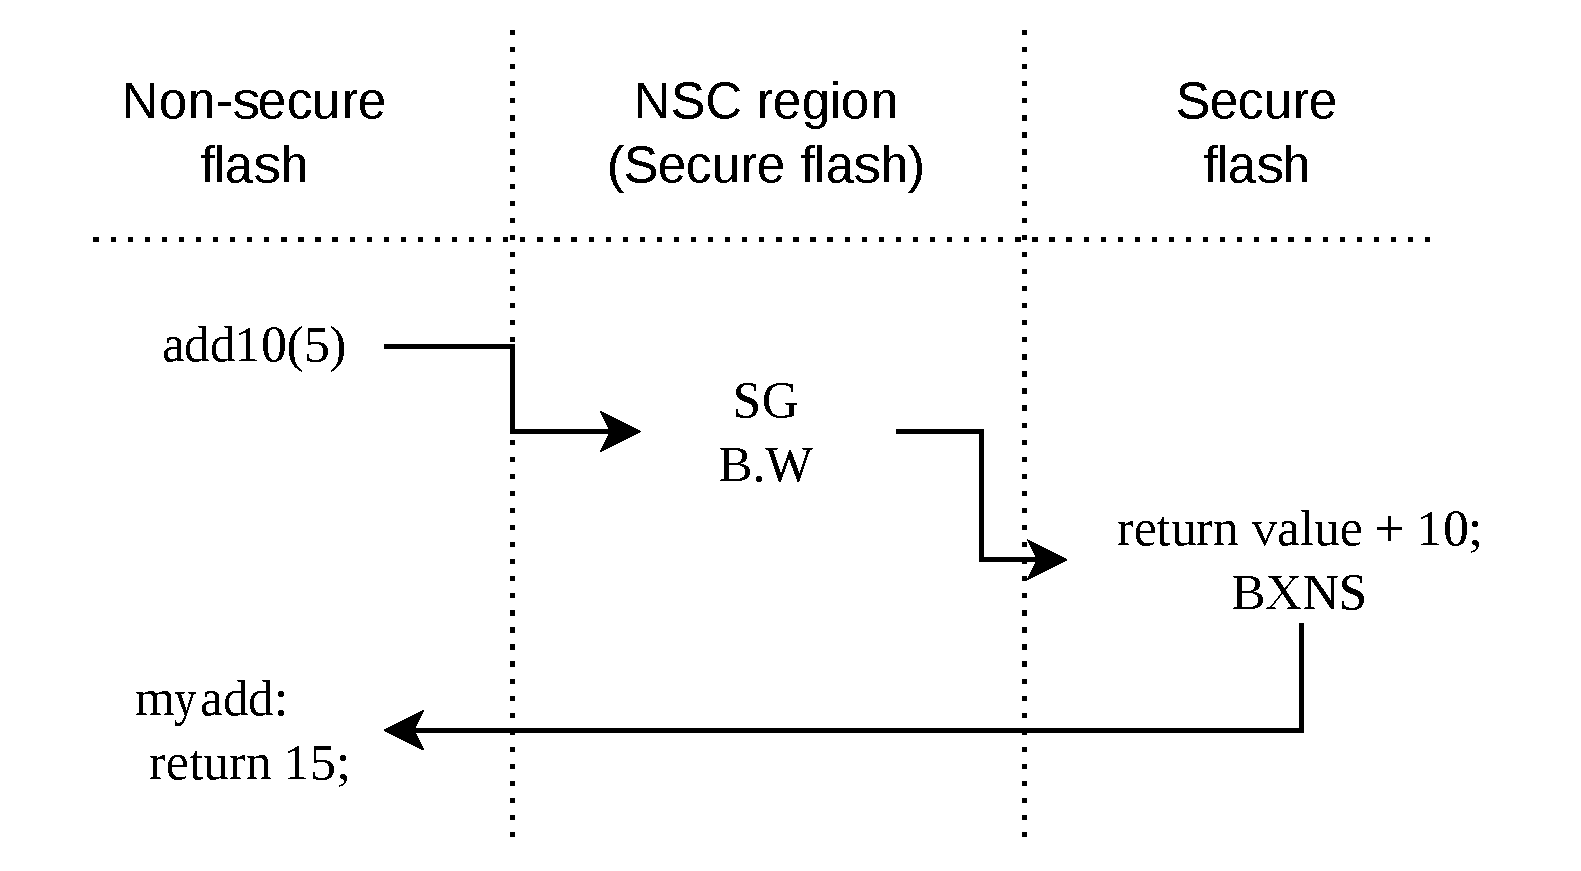
\includegraphics[width=\columnwidth]{graphics/microhastee-life-cycle.drawio.pdf}
  \caption{Control flow of a Non-secure call to a Secure entry function.
  The \texttt{SG} instruction in the NSC gateway veneer changes the processor to Secure state, after which \texttt{B.W} branches to the Secure function body.
  The function returns directly to its Non-secure caller with \texttt{BXNS}.}
  \Description{A three-column diagram shows a call from Non-secure flash entering an SG and B.W gateway veneer in an NSC region, executing the add10 function in Secure flash, and returning directly to the Non-secure caller with BXNS.}
  \label{fig:nsc-call}
\end{figure}

A Secure entry function must treat pointer arguments received from Non-secure code as untrusted.
Before dereferencing a pointer, it must verify that the entire referenced range lies in Non-secure memory, has the permissions required by the operation, and does not wrap around the address space when its size is added.
After validating an input range, Secure code copies its contents into Secure memory and performs subsequent checks and computations on that copy, preventing later modifications to the original buffer from changing the value being processed.

This section describes several relatively small mechanisms.
The difficulty arises when they need to be used together to agree on a security policy.
The simple act of allowing a Non-secure button handler to call a Secure service involves peripheral and interrupt attribution, a Non-secure vector entry, matching declarations in two programs, a gateway veneer, and an ordered build in which the Secure link produces input to the Non-secure link.
Each mechanism may by itself look correct, while some other part of the system disagrees with the policy.

\section{MicroHasTEE}

MicroHasTEE is a multitier programming framework in which the Secure and Non-secure applications are participants in one source-level program.
The program describes each participant's computations, the resources assigned to it, and the interactions permitted between the participants.
The build compiles this program twice, once for each TrustZone domain.
In the Secure build, \inlinehaskell{Secure} computations execute while \inlinehaskell{Nonsecure} computations are represented by placeholders; the Non-secure build reverses these roles.
The two builds select different implementations of the same MicroHasTEE interface, so they type-check the same setup sequence and derive corresponding views of the shared program.
The program's setup phase assigns security attribution, configures peripherals, registers callbacks and Secure services, and starts the Non-secure application.

MicroHasTEE represents resource ownership with a pair of type-level capability ledgers, one for each participant.
The \inlinehaskell{Setup} monad describes a transition from one pair of ledgers to another.

\begin{lstlisting}[style=haskell]
  data Setup nsPre sPre nsPost sPost a
\end{lstlisting}

The parameters \inlinehaskell{nsPre} and \inlinehaskell{sPre} describe the Non-secure and Secure ledgers before the setup computation.
The parameters \inlinehaskell{nsPost} and \inlinehaskell{sPost} describe the corresponding ledgers afterward.
The final parameter, \inlinehaskell{a}, denotes the value returned by the computation.
Each public attribution operation updates the hardware configuration and performs the corresponding transition between ledger pairs.
Assuming a correct hardware backend and no access through raw C, FFI, or internal interfaces, the final pair therefore describes the attribution established during setup.
Subsequent MicroHasTEE operations require evidence that their resource occurs in the executing participant's ledger, so the compiler rejects operations for which that participant lacks authority.

The configuration phase always begins with MicroHasTEE program being \textit{open to configuration}.\footnote{
For readability, the listings in this section abbreviate the type-level list representation with promoted-list syntax, such as \texttt{'[GPIO 7 C]}, rather than the \texttt{Cons (GPIO 7 C) Nil} representation used by the current MicroHs implementation.
They also write \texttt{Setup} computations with ordinary \texttt{do} notation, whereas the implementation uses \texttt{QualifiedDo} and \texttt{Ix.do} because \texttt{Setup} is an indexed monad.}
This is encoded by the capability ledger for the Secure domain carrying a \inlinehaskell{Unlocked} entry.
Consider the program below

\begin{lstlisting}[style=haskell]
  configure :: Setup '[] '[Unlocked] '[UART] '[Locked] ()
  configure = do
    uart <- get_console
    -- configuration of the actual UART device omitted
    tzsc_release_periph uart
    lock_configuration
\end{lstlisting}

The type of \inlinehaskell{configure} says that initially, the Non-secure application have no capabilities and the Secure capabilities indicate that MicroHasTEE is open for configuration.
The final ledgers assign the UART to the Non-secure participant and leave the Secure participant with no tracked peripheral capabilities.
The \inlinehaskell{Locked} entry records that further configuration is prohibited.
The intermediate types show the history of what happens with the type of the function

\begin{lstlisting}[style=haskell]
                 -- Initially ns = [],     s = [Unlocked]
  uart <- get_console      -- ns = [],     s = [UART, Unlocked]
  tzsc_release_periph uart -- ns = [UART], s = [Unlocked]
  lock_configuration       -- ns = [UART], s = [Locked]
\end{lstlisting}

The capability ledgers are used to enforce that certain things happens only when they are allowed.
For instance, MicroHasTEE requires that the UART is configured \textit{while it belongs to the Secure domain}.
Between line 3 and 5 in the \inlinehaskell{configure} function MicroHasTEE allows the UART to be configured.
The program below is rejected by the compiler as ill-formed, as the UART is configured \textit{after} it has been released to the Non-secure domain.

\begin{lstlisting}[style=haskell]
  configure :: Setup '[] '[Unlocked] '[UART] '[Locked] ()
  configure = do
    uart <- get_console

    tzsc_release_periph uart
    uart_init uart $ UARTConfig { baudrate    = 115200
                                , word_length = 8
                                , stop_bits   = 1
                                , parity      = NONE
                                }

    lock_configuration
\end{lstlisting}

\inlinehaskell{uart_init} requires both \inlinehaskell{Unlocked} and \inlinehaskell{UART} to be present in the Secure capability ledger.
At this point, the Secure ledger is \inlinehaskell{'[Unlocked]}.
Configuration remains open, but the UART is no longer available to Secure code, so the second constraint cannot be satisfied.

Acquiring a resource requires it to be absent from both ledgers.
After \inlinehaskell{tzsc_release_periph}, \inlinehaskell{UART} is absent from the Secure ledger but remains present in the Non-secure ledger.
The second \inlinehaskell{get_console} call is therefore rejected by the compiler.

\begin{lstlisting}[style=haskell]
  configure :: Setup '[] '[Unlocked] '[UART] '[UART, Unlocked] ()
  configure = do
    uart <- get_console
    tzsc_release_periph uart
    uart <- get_console
\end{lstlisting}

The restrictions demonstrated so far ensure that setup maintains a consistent account of what the security attribution on the hardware looks like.
The ledger stops representing the attribution of the program if the user can change it \textit{after} we have install callbacks or invoked the application.
MicroHasTEE therefore provides a one-way transition that finalizes the capability ledger, disallowing any future modification.

\begin{lstlisting}[style=haskell]
  lock_configuration :: ( Member Unlocked s
                        , Delete Unlocked s s')
                     => Setup ns s ns (Locked ': s') ()
\end{lstlisting}

The type of \inlinehaskell{lock_configuration} says that if the Secure ledger contained the element \inlinehaskell{Unlocked}, the Secure ledger is transformed to one that doesn't contain it, and instead contains \inlinehaskell{Locked}.
All operations that configure the device and change the ledger are gated on the presence of the \inlinehaskell{Unlocked} element in the Secure capability ledger.
Furthermore, the operations that install callbacks or denote Secure functions as callable from the Non-secure domain are similarly gated, and require a program where further configuration has been ruled out.
This act of locking the configuration phase is purely a type-level transition, and not something represented by a corresponding hardware action.
The program below is rejected by the compiler, as the red LED is requested after \inlinehaskell{lock_configuration} was invoked.

\begin{lstlisting}[style=haskell]
  bad = do
    lock_configuration
    red <- get_gpio @2 @G -- rejected
\end{lstlisting}

Finalizing setup produces the ledgers against which the two participant computations are checked.
MicroHasTEE represents these computations with the \inlinehaskell{Secure} and \inlinehaskell{Nonsecure} monads.

\begin{lstlisting}[style=haskell]
  data Secure    effects a
  data Nonsecure effects a
\end{lstlisting}

Peripheral operations are overloaded across these monads.
For example, \inlinehaskell{gpio_toggle} is a method of the \inlinehaskell{GPIOActions} class.

\begin{lstlisting}[style=haskell]
  class GPIOActions m where
    gpio_toggle :: Member (GPIO pin port) effects
                => GPIO pin port -> m effects ()
\end{lstlisting}

MicroHasTEE provides \inlinehaskell{GPIOActions} instances for both \inlinehaskell{Secure} and \inlinehaskell{Nonsecure}.
In either instance, the \inlinehaskell{Member} constraint requires the GPIO pin to occur in the capability ledger attached to the selected monad.
The same operation can therefore be used by either participant, but only when that participant has authority over the pin.
Consider the two programs below

\begin{lstlisting}[style=haskell]
  goodNonsecure :: GPIO 7 C -> Nonsecure '[GPIO 7 C] ()
  goodNonsecure pin = gpio_toggle pin

  badSecure :: GPIO 7 C -> Secure '[Locked, GPIO 2 G] ()
  badSecure pin = gpio_toggle pin
\end{lstlisting}

The compiler accepts \inlinehaskell{goodNonsecure} because its Non-secure ledger contains \inlinehaskell{GPIO 7 C}.
It rejects \inlinehaskell{badSecure} because its Secure ledger contains only \inlinehaskell{Locked} and \inlinehaskell{GPIO 2 G}, not \inlinehaskell{GPIO 7 C}.

With the underlying mechanisms MicroHasTEE uses to enforce correct security attribution explained, we next give an example of how to install a callback.
If the user has properly configured and attributed a GPIO device and its corresponding EXTI device, a callback can be installed against it.
When the underlying GPIO pin receives an edge transition, the installed callback is invoked.
Consider the function for installing a Non-secure callback below.

\begin{lstlisting}[style=haskell]
  exti_on_nonsecure :: (Member Locked s, Member (EXTI pin port) ns)
                    => EXTI pin port -> EXTIEdge -> (EXTIEdge -> Nonsecure ns ())
                    -> Setup ns s ns s ()
\end{lstlisting}

The type requires that in order to call this function, attribution must have been finalised (as evident by the \inlinehaskell{Locked} being present in the Secure capability ledger), and the interrupt belongs to the Non-secure participant.
Furthermore, the callback itself is a computation in the \inlinehaskell{Nonsecure} monad, whose list of effects unifies against the Non-secure capability ledger of the \inlinehaskell{Setup} monad.
This is a good point to reiterate why we lock down the configuration.
If unification is successfully done here against the capability ledger of the Non-secure domain, we don't want the program to proceed and make further configurations.
This will alter the capability ledger, making the guarantees provided by the prior unification moot.

So far we have described how security attribution is configured, and how callbacks are installed.
Crucially, we have not yet shown how the Non-secure domain can invoke secure services from the Secure domain.
This is done by explicitly registering \inlinehaskell{Secure} functions as \textit{callable}, and then providing a carefully typed interface for invoking them.
Consider the simple function below.

\begin{lstlisting}[style=haskell]
  add :: Int -> Int -> Secure effects Int
  add x y = return (x + y)
\end{lstlisting}

The function \inlinehaskell{add} takes two parameters and computes their sum in the \inlinehaskell{Secure} monad.
This function on its own cannot be invoked from the \inlinehaskell{Nonsecure} monad.
However, by marking it as \inlinehaskell{Callable}, we can.

\begin{lstlisting}[style=haskell]
  callable :: (Member Locked s, NonSecureCallable s f)
           => f -> Setup ns s ns s (Callable f)

  (<.>) :: NFData a => Callable (a -> b) -> a -> Callable b
\end{lstlisting}

The \inlinehaskell{Member Locked s} constraint permits a Secure service to be registered only after setup has been finalized.
The \inlinehaskell{NonSecureCallable s f} constraint accepts a Secure computation over the effect ledger \inlinehaskell{s}, or a function of arbitrary arity that eventually produces such a computation.
It therefore unifies the service's effect ledger with the final Secure ledger carried by the surrounding \inlinehaskell{Setup} computation.
For programs expressed through the public interface, a registered service can consequently use only the resources retained by the Secure participant.

The \inlinehaskell{callable} function returns an opaque \inlinehaskell{Callable} handle through which the Non-secure participant may refer to the registered service.
The \inlinehaskell{<.>} operator applies one argument to such a handle while preserving the remaining function type.

\begin{lstlisting}[style=haskell]
  f <- callable add
  let g = f <.> 10 <.> 5
\end{lstlisting}

The type of \inlinehaskell{f} is \inlinehaskell{Callable (Int -> Int -> Secure effects Int)}, while the type of \inlinehaskell{g} is \inlinehaskell{Callable (Secure effects Int)}.
The type of \inlinehaskell{g} shows that both arguments have been supplied and that the service is ready to be invoked with \inlinehaskell{sg}.

\begin{lstlisting}[style=haskell]
  sg :: Callable (Secure s a) -> Nonsecure ns a
\end{lstlisting}

Given a fully applied handle, \inlinehaskell{sg} invokes the corresponding Secure computation and returns its result in the \inlinehaskell{Nonsecure} monad.
The function \inlinehaskell{sg} has quite a straight-forward type.
Within MicroHasTEE's public Haskell interface, \inlinehaskell{sg} is the only operation that transfers explicit argument and result values between the participants.
When the call is made the parameters are passed from the Non-secure domain to the Secure domain, and when the result is returned it is passed from the Secure domain to the Non-secure domain.

Finally, when te callbacks have been installed and the Secure services have been made callable, we invoke the Non-secure application.
This is done through the \inlinehaskell{nonsecure} function.
\todo{I should see if I cannot change the code to allow invokaton of nonsecure to happen only once...}

\begin{lstlisting}[style=haskell]
  nonsecure :: Member Locked s
            => Nonsecure ns () -> Setup ns s ns s ()
\end{lstlisting}

The type states that if the attribution phase has been locked down, we can run the Non-secure application.

A small example of a complete application is shown below.

\begin{lstlisting}[style=haskell]
  {-# LANGUAGE DataKinds #-}
  {-# LANGUAGE TypeApplications #-}

  module BlinkExample where

  import MicroHasTEE

  type NSEffects = '[GPIO 7 C]
  type SEffects = '[Locked, GPIO 2 G]

  toggleLED :: GPIO 2 G -> Secure SEffects ()
  toggleLED = gpio_toggle

  loop :: GPIO 7 C
       -> Callable (Secure SEffects ())
       -> Nonsecure NSEffects ()
  loop green toggle = do
    gpio_toggle green
    sg toggle
    systick_delay_ms 500
    loop green toggle

  app :: Setup '[] '[Unlocked] NSEffects SEffects ()
  app = do
    board_init
    board_configure_pll
    hz <- board_sysclk_hz
    systick_configure (hz `div` 1000)

    rcc <- get_rcc
    rcc_enable rcc RCC_GPIOG
    rcc_enable rcc RCC_GPIOC

    let output = GPIOConfig { mode = OUTPUT
                            , pull = NOPULL
                            , alternate = AF0
                            }

    red <- get_gpio @2 @G
    gpio_init red output

    green <- get_gpio @7 @C
    gpio_init green output
    gpio_release green

    lock_configuration
    toggle <- callable (toggleLED red)
    nonsecure (loop green toggle)

  main :: IO ()
  main = runSetup app
\end{lstlisting}

The Non-secure loop toggles the green LED directly and toggles the red LED by invoking the registered Secure function through \inlinehaskell{sg}.
The red LED belongs to the Secure domain, and can only be manipulated by the Secure application.

MicroHs generates one C source file from each of the two builds.
The build system compiles and links each generated file with the MicroHs runtime, startup code, C glue code, and the drivers for its domain to produce the corresponding firmware image.

For programs expressed through its public interface, MicroHasTEE prevents duplicate acquisition, use without ledger authority, configuration after finalization, callbacks attached to the wrong participant, and calls to Secure functions that were not explicitly registered.
These guarantees rely on the MicroHasTEE implementation, its hardware backend, and the deployment of matching firmware images.
Raw C, FFI, internal interfaces, and malformed gateway input remain outside the static model.

\section{Implementation}
\label{sec:implementation}

\section{Evaluation}

\section{Related Work}

MicroHasTEE is inspired by HasTEE, a Haskell framework for confidential computing on Intel SGX.
The multiparty programming model and implementation is inspired by HasTEE, but whereas MicroHasTEE is executing in TrustZone-M on an MCU, HasTEE executed in Intel SGX enclaves on larger machines, such as laptops.
Furthermore, to run Haskell in the enclave HasTEE used a patched version of the GHC runtime system.
MicroHasTEE is compiling and running the upstream version of the MicroHs runtime system and deploys that in TrustZone-M.

\todo{rust for TrustZone-M}.

There are relatively few projects where a high-level managed language like Haskell is used to run code in TrustZone-M.
If we instead divert our eyes to TrustZone-A or Intel SGX, we find more projects.

GoTEE\todo{cite} is a project where a Go compiler and runtime was heavily modified to suppoert \textit{secure routines}, which are executed inside enclaves.
Furthermore, GoTEE implements channels for communication between the enclave and the program running outside.
The Go compiler was extended with support for automatically partitioning a program, but does otherwise not help the programmer control how sensitive data moves within a program.

J\(_{E}\) implements a subset of Java, and comes with support for running in enclaves.
It uses Information-Flow Control to ensure that data does not flow through the program in undesireble ways.
Compilation is advanced, with a program first undergoing partitioning before another pass ensures that the two programs interactions are not ill-formed.


\section{Conclusions \& Future Work}

MicroHasTEE can reliably reject a whole class of attribution-related bugs, turning runtime errors into compile-time errors.
We have shown that a high-level functional language can be used to program resource-constrainted MCUs, as well as running it in TrustZone-M.

Evaluation\todo{yet to be done} shows that there is a significant performance cost associated with using MicroHasTEE.
The prototype is compiled with a non-optimising compiler, and deployed to a runtime that uses a simple but small bytecode interpreter.
For these reasons we are not surprised by the results.
A more mature implementation of MicroHasTEE should strive to use a more efficient runtime, but none exists today.

%%
%% The acknowledgments section is defined using the "acks" environment
%% (and NOT an unnumbered section). This ensures the proper
%% identification of the section in the article metadata, and the
%% consistent spelling of the heading.
\begin{acks}
  I would like to thank large-language-Joel for always answering any embedded question I have, and Lennart Augustsson.
\end{acks}

%%
%% The next two lines define the bibliography style to be used, and
%% the bibliography file.
\bibliographystyle{ACM-Reference-Format}
\bibliography{main}


%%
%% If your work has an appendix, this is the place to put it.
\appendix

\end{document}
\endinput
%%
%% End of file `sigconf.tex'.
